\documentclass[utf8,xcolor=table]{beamer}

\usepackage[T2A]{fontenc}
\usepackage[utf8]{inputenc}
\usepackage[english,russian]{babel}
\usepackage{tikz}
\usetikzlibrary{shapes,arrows}
\usepackage{dot2texi}
\usepackage{minted}
\usepackage{ulem}
\usepackage{cmap}
\usepackage{multirow}

\hypersetup{colorlinks,linkcolor=blue,urlcolor=blue}

\mode<presentation>{
	\usetheme{CambridgeUS}
}

\renewcommand{\t}[1]{\ifmmode{\mathtt{#1}}\else{\texttt{#1}}\fi}

\title{Типы в Haskell}
\author{Егор Суворов}
\institute[СПб АУ]{Курс <<Парадигмы и языки программирования>>, подгруппа 3}
\date[09.11.2016]{Среда, 9 ноября  года}

\setlength{\arrayrulewidth}{1pt}

\begin{document}

\begin{frame}
\titlepage
\end{frame}

\begin{frame}{План занятия}
	\tableofcontents
\end{frame}

\section{Ещё про Haskell}
\subsection{Функции высшего порядка}

\begin{frame}
	\tableofcontents[currentsection,currentsubsection]
\end{frame}

\begin{frame}{Напоминание}
	\begin{itemize}
		\item Функция является \textit{функцией высшего порядка}, если она в качестве одного из аргументов принимает другую функцию.
		\item Пример: \t{map}. Он первым параметром принимает функцию, которая преобразует элементы списка.
		\item Пример: \t{dropWhile}. Первый аргумент умеет по элементу сообщать, надо остановиться или нет.
		\item Пример: \t{filter cond list}. Оставляет в списке только элементы, удовлетворяющие условию.
		\item Функции высшего порядка является основными кирпичиками в функциональном программировании.
	\end{itemize}
\end{frame}

\begin{frame}[fragile]{Ещё один паттерн}
\begin{minted}{haskell}
sum (x:xs) = x + sum xs
sum _ = 0

prod (x:xs) = x * prod xs
prod _ = 1

max (x:xs) = max x (max xs)
max x = -1

concat (x:xs) = x ++ (concat xs)
concat _ = ""
\end{minted}
	Что общего?
	\pause
	\begin{itemize}
		\item Все эти функции считают функцию от множества элементов.
		\item Для пересчёта требуется знать только текущее значение и очередной элемент.
	\end{itemize}
\end{frame}

\begin{frame}[t,fragile]{Правая свёртка}
\begin{minted}{haskell}
foldr f a (x:xs) = f x (foldr f a xs)
foldr f a _ = a

sum    xs = foldr (+)  0    xs
prod   xs = foldr (*)  1    xs
max    xs = foldr max  (-1) xs
concat xs = foldr (++) ""   xs
\end{minted}
	Ещё одна популярная функция высшего порядка.
\end{frame}

\begin{frame}[fragile]{Упражнение на понимание}
\begin{minted}{haskell}
foldr f a (x:xs) = f x (foldr f a xs)
foldr f a _ = a
\end{minted}

	А что такое \t{foldr (:) [4,5] xs}?
	\pause
\begin{minted}{haskell}
foldr (:) [4,5] [1,2,3] =
1:(foldr (:) [4,5] [2,3]) =
1:(2:(foldr (:) [4,5] [3])) =
1:(2:(3:(foldr (:) [4,5] []))) =
1:(2:(3:[4,5])) =
[1,2,3,4,5]
\end{minted}
	Дописывание \t{[4,5]} в конец списка.

\begin{minted}{haskell}
(++) a b = foldr (:) b a
\end{minted}
\end{frame}

\begin{frame}{Картинка}
	\begin{center}
		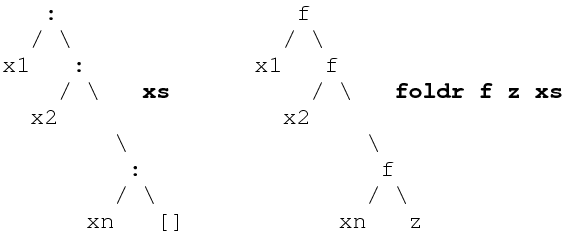
\includegraphics[scale=0.5]{foldr.png}
	\end{center}
	Бамбук растёт вправо, поэтому \textit{правая} свёртка.
\end{frame}

\begin{frame}[fragile]{Упражнения}
	Как узнать, все ли элементы равны \t{True}? \pause
\begin{minted}{haskell}
foldr (&&) True xs
\end{minted}

	Как узнать сумму квадратов чисел в массиве? \pause
\begin{minted}{haskell}
foldr (+) 0 (map (^2) xs)
\end{minted}

	Как выразить \t{map} через \t{foldr}? \pause
\begin{minted}{haskell}
map f xs = foldr (\a x -> (f a):x) [] xs
\end{minted}
	Вывод: в теории почти всё есть \t{foldr}.
	На практике лучше использовать готовые функции.
\end{frame}

\subsection{Статический полиморфизм функций}

\begin{frame}
	\tableofcontents[currentsection,currentsubsection]
\end{frame}

\begin{frame}
	\begin{itemize}
		\item Мы нигде не указывали типы ни аргументов функций, ни возвращаемых значений.
		\item Свободно использовали функции для разных типов (вроде \t{map}).
		\item Если набрать \t{:t map} в GHCI, увидим её тип:
		\[
			\t{\underbrace{(a~->~b)}_{\text{функция}}~->~\underbrace{[a]}_{\text{исходный список}}~->~\underbrace{[b]}_{\text{результат}}}.
		\]
		\item Справа от последней \t{->} "--- возвращаемое значение, до этого "--- аргументы.
		\item Тут \t{a} и \t{b} "--- типовые переменные. На их месте может стоять любой тип.
		\item Естественным образом получаем, что \t{map} вообще всё равно, с какими списками работать.
		\item Haskell автоматически выводит наиболее общие типы для практически всех функций.
		\item Все проверки типов "--- \textit{на этапе компиляции}.
	\end{itemize}
\end{frame}

\begin{frame}{Что могут делать функции}
	\begin{itemize}
		\item Что вообще может делать \textit{чистая} функция с типом \t{Bool~->~Bool}?
		\item Их всего $2^2=4$ различных: всегда \t{True}, всегда \t{False}, отрицание, тождественная.
		\item А что может делать полиморфная функция с типом \t{a~->~a}? \pause
		\item Только возвращать свой аргумент "--- она не имеет права ничего про него предполагать. \pause
		\item А функции с типом \t{a~->~b} не бывает "--- она в общем случае не может создать что-то типа \t{b}.
		\item Что может делать \t{a~->~[a]}? \pause
		\item Только создавать список из одинаковых элементов \textit{фиксированной} длины, которая не зависит от аргумента.
	\end{itemize}
\end{frame}

\begin{frame}{Игра}
	Ваша задача "--- по типу функции угадать, что она делает.
	\begin{tabular}{c|c}
		\centering
		Тип & Функция \\\hline
		\t{a -> a} & \pause\t{id x = x} \\\pause
		\t{a -> b -> a} & \pause\t{fst x y = x} \\\pause
		\t{a -> b -> b} & \pause\t{snd x y = y} \\\pause
		\t{(a -> b) -> a -> b} & \pause\t{apply f x = f x} \\\pause
		\t{[a] -> a} & \pause\t{get xs = xs !! c} \\\pause
		\t{(a -> Bool) -> [a] -> [a]} & \pause\t{filter} \\\pause
		\t{(a -> Bool) -> [a] -> [a]} & \pause\t{dropWhile} \\\pause
		\t{(a -> Int) -> [a] -> Int} & \pause\t{sum (map f xs)} \\\pause
		\t{(a -> b -> b) -> b -> [a] -> b} & \pause\t{foldr}
	\end{tabular}
\end{frame}

\begin{frame}{Вывод типов}
	Ваша задача "--- по определению функции вывести наиболее общий тип.
	\begin{tabular}{c|c}
		\centering
		Функция & Тип \\\hline
		\t{foo x y = x y} & \pause \t{(a -> b) -> a -> b} \\\pause
		\t{foo x y z = x y z} & \pause \t{(a -> b -> c) -> a -> b -> c} \\\pause
		\t{foo x y z = (x y) + (x z)} & \pause \t{(a -> Int) -> a -> a -> Int} \\\pause
		\t{foo x y = (x y) + y} & \pause \t{(Int -> Int) -> Int -> Int} \\\pause
		\t{foo x y = (x y):y} & \pause \t{([a] -> a) -> [a] -> [a]} \\
	\end{tabular}
\end{frame}

\begin{frame}{Резюме}
	\begin{itemize}
		\item Без полиморфизма функции высшего порядка были бы бесполезны.
		\item Часто по типу полиморфной функции можно догадаться, что она делает.
		\item Есть специальный поисковик \href{https://www.haskell.org/hoogle/}{Hoogle}, который ищет функции по их типу.
		\item Hoogle "--- полезная штука, если вам нужна какая-то <<очевидно полезная>> функция. Найдётся всё.
	\end{itemize}
\end{frame}

\section{Алгебраические типы данных}
\subsection{Откуда берётся тип-сумма}

\begin{frame}
	\tableofcontents[currentsection,currentsubsection]
\end{frame}

\begin{frame}{Тип-произведение}
	\begin{itemize}
		\item \t{int x;} принимает значения: $0, 1, -1, 2, -2, \dots$
		\item \t{struct \{ int x, y; \} } принимает значения: $(0, 0), (0, 1), (1, 0), (-1, 0) \dots$
		\item Множество значений \t{struct} есть декартово произведение значений составных элементов.
		\item Поэтому \t{struct} иногда называют типом-произведением.
		\item Тип-произведение "--- \textit{составной тип}, собирается из более маленьких.
		\item Есть практически во всех языках.
	\end{itemize}
\end{frame}

\begin{frame}{Упражнение}
	\begin{itemize}
		\item Пусть у интернет-магазина есть три способа оплаты:
			\begin{enumerate}
				\item Банковской картой, нужно знать её данные.
				\item Наличными при получении, ничего дополнительно знать не нужно.
				\item Выставление счёта на QIWI-кошелёк, нужно знать номер телефона.
			\end{enumerate}
		\item Требуется создать тип данных <<способ оплаты>>, который можно хранить и обрабатывать.
		\item Иногда требуется преобразовывать способ оплаты в строку.
		\item Иногда требуется понимать, надо ли что-то делать с сервере для проведения оплаты (если да "--- положить в очередь).
	\end{itemize}
\end{frame}

\begin{frame}[fragile]{Упражнение (C-подход)}
\begin{minted}{cpp}
enum PaymentMethodType { CARD, CASH, QIWI_BILL };
struct PaymentMethod {
  PaymentMethodType type;
  CardInfo card_info;
  char phone[20];
};
\end{minted}
	\begin{itemize}
		\item Надо везде явно смотреть на поле \t{type} и городить if'ы.
		\item Для обработки пишем функции вроде \t{to\_string}, которые разбирают случаи.
		\item Можем случайно обратиться к \t{card\_info}, если не проверим способ оплаты.
		\item Храним больше байт, чем реально надо (можно \t{union}, но там есть свои проблемы).
	\end{itemize}
\end{frame}

\begin{frame}{Упражнение (ООП-подход)}
	\begin{itemize}
		\item Вводим интерфейс \t{PaymentMethod}, а сами методы делаем подклассами.
		\item Общие функции вроде \t{to\_string} вносим в интерфейс.
		\item Специфичные функции либо руками разбирают случаи, либо используют Visitor.
		\item Так обычно и делают.
		\item Можно добавлять как новые классы, так и новые операции с объектами.
	\end{itemize}
\end{frame}

\subsection{Что такое тип-сумма}
\begin{frame}[fragile]{Тип-сумма}
	\begin{itemize}
		\item Можно ввести \textit{тип-сумму}: множество его допустимых значений равно \textit{дизъюнктному объединению}\footnote{объединение попарно непересекающихся множеств} допустимых значений составных частей.
		\item Чтобы обобщить до суммы произвольных типов, можно каждому значению составной части добавить <<тэг>>.
		\item Пример: тип <<способ оплаты>>:
\begin{minted}{haskell}
data PaymentMethod = BankCard String | Cash | Qiwi String
a = BankCard "1234 5678 9012 3456"
b = Cash
c = Qiwi "+7 812 000 00 00"
\end{minted}
		\item Обычно встречается в функциональных языках.
		\item Именно его наличие обычно подразумевают под <<наличием алгебраических типов данных>>.
	\end{itemize}
\end{frame}

\begin{frame}[fragile]{Тип-сумма: подробности}
\begin{minted}{haskell}
data PaymentMethod = BankCard String | Cash | Qiwi String
\end{minted}
	\begin{itemize}
		\item \t{PaymentMethod} называется \textit{конструктором типа}.
		\item \t{BankCard}, \t{Cash}, \t{Qiwi} называются <<конструкторами данных>>, являются теми самыми <<тэгами>>.
		\item Не путать с конструкторами в ООП!
		\item И конструктор типа, и конструктор данных долнжы начинаться с большой буквы.
		\item Работает с pattern matching:
\begin{minted}{haskell}
to_string (BankCard num) = "BankCard " ++ num
to_string Cash           = "Cash"
to_string (Qiwi phone)   = "Qiwi " ++ phone
\end{minted}
		\item Можно дописать в конец строки с \t{data} слова \t{deriving Show}, чтобы GHCI мог выводить значения типа \t{PaymentMethod}.
	\end{itemize}
\end{frame}

\subsection{Примеры типов-сумм}
\begin{frame}
	\tableofcontents[currentsection,currentsubsection]
\end{frame}

\begin{frame}[fragile]{CharOrNotFound}
	Поиск элемента по номеру:
\begin{minted}{haskell}
data CharOrNotFound = NotFound | Found Char deriving Show

getItem :: [Char] -> Int -> CharOrNotFound
getItem (x:_ ) 0         = Found x
getItem (x:xs) n | n > 0 = getItem xs (n - 1)
getItem _      _         = NotFound
\end{minted}
	\begin{itemize}
		\item Не требуются <<магические значения>> для ситуации <<элемент не найден>>.
		\item Компилятор проверяют, что мы всегда обрабатываем оба случая.
		\item По типу функции сразу понятно, что она может вернуть.
		\item Нет исключений; функции чистые.
	\end{itemize}	
\end{frame}


\begin{frame}[fragile]{Maybe}
	Можно обобщить до \textit{параметризованного типа}:
\begin{minted}{haskell}
data GetResult a = NotFound | Found a deriving Show

getItem :: [a] -> Int -> GetResult a
getItem (x:_ ) 0         = Found x
getItem (x:xs) n | n > 0 = getItem xs (n - 1)
getItem _ _              = NotFound
\end{minted}
% Показать :t getItem, :t getItem "123" 1
	\begin{itemize}
		\item \t{GetResult} "--- это не тип, это \textit{конструктор типа}.
		\item \t{a} "--- единственный параметр этого конструктора.
		\item А вот \t{GetResult Char} "--- уже конкретный тип:
\begin{minted}{haskell}
data GetResult Char = NotFound | Found Char
\end{minted}
		\item В Haskell такой тип называется (\t{Maybe}.
		\item А в Java есть generic-тип \t{Optional<>}).
		\item На самом деле \t{[Int]} "--- это сахар для \t{[] Int}.
	\end{itemize}
\end{frame}

\begin{frame}[t,fragile]{Упражнение}
	\begin{itemize}
		\item Напишите тип для функции \t{getItem}, если бы она использовала \t{Maybe}:
\begin{minted}{haskell}
-- Уже объявлен в языке, писать не надо.
data Maybe a = Nothing | Just a

getItem :: [a] -> Int -> ???
\end{minted}
		\item Напишите функцию \t{getItem}.
		\item Удалите явное указание типа, проверьте, какой тип вывелcя автоматически (\t{:t getItem} в GHCI).
	\end{itemize}
	\pause
\begin{minted}{haskell}
getItem :: [a] -> Int -> Maybe a
getItem (x:_)  0         = Just x
getItem (x:xs) n | n > 0 = getItem xs (n - 1)
getItem _ _              = Nothing
\end{minted}
\end{frame}

\begin{frame}[fragile]{Either}
	На случай, если хотим сообщить об ошибке:
\begin{minted}{haskell}
-- Уже объявлен в языке, писать не надо.
data Either a b = Left a | Right b

parseBool :: String -> Either String Bool
parseBool "true"  = Right True
parseBool "false" = Right False
parseBool x       = Left ("Invalid value: " ++ x)
\end{minted}
	\begin{itemize}
		\item Обычно за \t{Right} принимает успешное вычисление (<<правильный>> результат).
		\item А за \t{Left} "--- сообщение об ошибке (<<левый>> результат).
	\end{itemize}
\end{frame}

\begin{frame}[fragile]{Двоичная куча}
\begin{minted}{haskell}
data Heap = Nil | Node Int Heap Heap deriving Show

Node 1 (Node 2 (Node 5 (Node 6 Nil Nil) Nil)
               (Node 4 Nil Nil))
       (Node 3 Nil Nil)
\end{minted}
	\begin{center}
		\begin{dot2tex}[scale=0.5,options=-tmath]
			graph G {
			    1 {rank=same 2 3} {rank=same 5 4} { rank=same 6 x }
			    1 -- {2 3};
			    2 -- {5 4};
			    5 -- 6;
			    5 -- x [style=invis];
			    x [style=invis];
			}
		\end{dot2tex}
	\end{center}
\end{frame}

\begin{frame}[fragile]{Min-Max куча}
	Так как вершина всегда хранит либо минимум, либо максимум, это можно указать прямо в типе.
	Тогда точно не запутаемся, где какая вершина, и не надо это явно считать и передавать.
\begin{minted}{haskell}
data MinMaxHeap = Nil | MinNode Int MinMaxHeap MinMaxHeap
                      | MaxNode Int MinMaxHeap MinMaxHeap
\end{minted}
	Можно даже строже, у нас есть взаимная рекурсия:
\begin{minted}{haskell}
data MinMaxHeap = Nil1 | MinNode Int MaxMinHeap MaxMinHeap
data MaxMinHeap = Nil2 | MaxNode Int MinMaxHeap MinMaxHeap
\end{minted}	
	К сожалению, назвать оба конструктора данных \t{Nil} нельзя.
\end{frame}

\begin{frame}[fragile]{Односвязные списки}
\begin{minted}{haskell}
data List a = Empty | Cons a (List a) deriving Show

head' (Cons x _ ) = x
tail' (Cons _ xs) = xs
\end{minted}
	\begin{itemize}
		\item Выше написано почти определение встроенного списка.
		\item \t{[]} "--- это сахар для конструктора \t{Empty}.
		\item \t{:} "--- это сахар для конструктора \t{Cons}.
		\item Конкретно в Haskell любые структуры бывают бесконечными из-за ленивости, не только списки.
		\item Например, бесконечное двоичное дерево имеет право на жизнь.
	\end{itemize}
\end{frame}

\begin{frame}[fragile]{Упражнение}
	\begin{enumerate}
		\item Напишите тип <<двоичное дерево>> (\t{Tree}), в котором у каждой вершины либо 0 детей, либо 2, а каждая вершина содержит значение типа \t{Int}.
		\item Добавьте \t{deriving Show}.
		\item Напишите функцию \t{tree\_sum}, которая считает сумму в данном ей дереве.
		\item Удалите разбор какого-нибудь случая и запустите GHCI так: \t{ghci~-W~file.hs}
		\item Убедитесь, что выпало предупреждение о неразобранном случае.
		\item Напишите функцию, которая возвращает бесконечное дерево \t{Int}'ов, где каждая вершина содержит номер своего уровня.
		\item Выведите результат на экран, объясните увиденное.
	\end{enumerate}
\end{frame}

\begin{frame}{Промежуточные итоги}
	\begin{itemize}
		\item
			Под <<алгебраическими типами данных>> обычно подразумевают поддержку типов-сумм вместе с типами-произведениями \textit{на уровне языка}.
			Такая поддержка даёт:
			\begin{enumerate}
				\item Более наглядные типы.
				\item Невозможность обратиться к данным из другого <<случая>>.
				\item Pattern matching и сильное упрощение кода.
				\item Предупреждения компилятора о нерассмотренных случаях (ключ \t{-W} для GHC/GHCI).
			\end{enumerate}
		\item Добавлять случаи в тип-сумму обычно после объявления нельзя.
		\item В языках без типов-сумм, но с ООП, обычно используется:
			\begin{itemize}
				\item Наследование от общего предка вместо типов-сумм.
				\item Visitor вместо pattern mactching.
			\end{itemize}
		\item Типы-суммы очень часто возникают при работе с AST.
		\item В Haskell любой пользовательский тип является типом-суммой (возможно, из одного слагаемого).
		\item В Haskell можно параметризовать пользовательские типы.
	\end{itemize}
\end{frame}

\subsection{Использование типов-сумм}
\begin{frame}
	\tableofcontents[currentsection,currentsubsection]
\end{frame}

\begin{frame}[t,fragile]{Хранение URL}
	URL-адреса бывают:
	\begin{itemize}
		\item Относительные: \t{../images/facepalm.jpg}.
		\item Абсолютные, бывают:
			\begin{itemize}
				\item На том же домене: \t{sewiki/index.php}.
				\item На другом домене, причём:
					\begin{itemize}
						\item Та же схема (протокол): \t{google.com/humans.txt}
	                    \item Другая схема: \t{ftp://mirror.yandex.ru/}
                   	\end{itemize}
			\end{itemize}
	\end{itemize}
\begin{onlyenv}<1>
	Можно закодировать так\footnote{True story: раздел <<Thinking in Sum Types>> по \href{https://chadaustin.me/2015/07/sum-types/}{ссылке}}:
\begin{minted}{haskell}
data URL = URL (Maybe (Maybe (Maybe String, String))) String
URL Nothing        "../images/facepalm.jpg"
URL (Just Nothing) "sewiki/index.php"
URL (Just (Just (Nothing   , "google.com"))) "humans.txt"
URL (Just (Just (Just "ftp", "mirror.yandex.ru"))) ""
\end{minted}
Ужасно, не правда ли?
\end{onlyenv}

\begin{onlyenv}<2>
А можно так:
\begin{minted}{haskell}
data URL = Relative String
         | Absolute String
         | OtherDomain { domain :: String, path :: String }
         | FullUrl     { schema :: String,
                         domain :: String, path :: String }
\end{minted}
Мораль: иногда может помочь <<раскрыть по дистрибутивности>>.
\end{onlyenv}
\end{frame}

\section{Классы типов}
\subsection{Что и зачем}

\begin{frame}
	\tableofcontents[currentsection,currentsubsection]
\end{frame}

\begin{frame}[fragile]{Pattern Matching и \t{==}}
\begin{minted}{haskell}
data IntList = Empty | Cons Int IntList deriving Show
a = Cons 1 (Cons 2 Empty)
b = Cons 1 (Cons 2 Empty)
c = Cons 1 (Cons 3 Empty)

isA :: IntList -> Bool
isA (Cons 1 (Cons 2 Empty)) = True
isA _                       = False

isA a -- True
isA b -- True
isA c -- False
a == b  -- ошибка компиляции?
a == c  -- ошибка компиляции?
\end{minted}
\end{frame}

\begin{frame}[fragile]{Eq}
	\begin{itemize}
		\item Pattern Matching "--- конструкция на уровне языка.
		\item \t{==} "--- просто некоторая функция с таким названием.
		\item В C++ мы бы написали перегрузку функции/оператора.
		\item В Haskell пишем так:
\begin{minted}{haskell}
instance Eq IntList where
  Empty       == Empty       = True
  (Cons x xs) == (Cons y ys) = (x == y) && (xs == ys)
  _           == _           = False

a == b  -- True
a == c  -- False
b == c  -- False
Empty == Empty           -- True
Empty /= (Cons 1 Empty)  -- True, /= тоже работает
\end{minted}
	\end{itemize}
\end{frame}

\begin{frame}[fragile]{class Eq}
	\begin{itemize}
		\item \t{Eq} "--- это \textit{класс типов}, который описывает, что к типам можно применять определённые функции:
\begin{minted}{haskell}
class Eq a where
  (==) :: a -> a -> Bool
  (/=) :: a -> a -> Bool
\end{minted}
		\item Говорим, что тип \t{a} лежит в классе \t{Eq} тогда и только тогда, когда для него есть функции \t{(==)} и \t{(/=)}
		\item Класс типов "--- это такой <<интерфейс>> для типов.
		\item Некоторые функции требуют, чтобы параметры были в определённых классах:
\begin{minted}{haskell}
lookup :: Eq a => a -> [(a, b)] -> Maybe b
\end{minted}
		\item Слово \t{instance} на предыдущем слайде добавляло \t{IntList} в класс \t{Eq}.
		\item Не путать с классами объектов из ООП!
	\end{itemize}
\end{frame}

\begin{frame}[fragile]{Реализации по умолчанию}
	\begin{itemize}
		\item Для \t{IntList} мы реализовали только \t{==}, а \t{/=} получили автоматом.
		\item В классе можно указывать реализацию по умолчанию:
\begin{minted}{haskell}
class Eq a where
  (==) :: a -> a -> Bool
  (==) a b = not (a /= b)
  (/=) :: a -> a -> Bool
  (/=) a b = not (a == b)
\end{minted}
		\item Тогда \textit{минимальное полное определение} для \t{Eq} "--- это либо \t{==}, либо \t{/=}.
	\end{itemize}
\end{frame}

\subsection{Для параметризованных типов}
\begin{frame}[fragile]{Класс Eq для списков}
	\begin{itemize}
		\item Пусть есть свой класс для списков:
\begin{minted}{haskell}
data List a = Empty | Cons a (List a)
\end{minted}
		\item Разумно считать, что списки равны, если равны элементы:
\begin{minted}{haskell}
instance Eq (List a) where
  Empty       == Empty       = True
  (Cons x xs) == (Cons y ys) = (x == y) && (xs == ys)
  _ == _                     = False
\end{minted}
		\item Не скомпилируется, потому что элементы произвольного типа \t{a} нельзя сранивать.
		\item Надо добавить \textit{контекст} "--- сказать, что списки можно сравнивать только если можно сранивать элементы:
\begin{minted}{haskell}
instance Eq a => Eq (List a) where
\end{minted}
	\end{itemize}
\end{frame}

\begin{frame}[fragile]{Классы для структур данных}
	\begin{itemize}
		\item Иногда хочется указать, что структура данных обладает некоторым свойством:
\begin{minted}{haskell}
class Mappable f where
  map' :: (a -> b) -> f a -> f b
\end{minted}
		\item \t{Mappable} "--- что-то, содержащее элементы произвольного типа, к чему можно делать \t{map'}.
		\item Можно реализовать:
\begin{minted}{haskell}
instance Mappable List where
  map' _ Empty = Empty
  map' f (Cons x xs) = Cons (f x) (map' f xs)

map' (+1) (Cons 1 (Cons 10 Empty))
-- Cons 2 (Cons 11 Empty)
\end{minted}
	\end{itemize}
\end{frame}

\begin{frame}[fragile]{Functor}
	\begin{itemize}
		\item Аналог \t{Mappable} в Haskell называется \t{Functor}, в нём определена функция \t{fmap}.
		\item \t{fmap} должна удовлетворять некоторым аксиомам, но их компилятор сам не проверит:
\begin{minted}{haskell}
fmap id x == x
fmap (f . g) x == fmap f (fmap g x)
\end{minted}
		\item После реализации \t{Functor} наш новый тип можно использовать в том числе в старых функциях:
\begin{minted}{haskell}
a = (Cons 1 (Cons 2 (Cons 3 Empty)))
fmap (+1) [1,2,3]
fmap (+1) a
-- Встроенный оператор замены значений на константу
10 <$ [1,2,3]  -- [10,10,10]
10 <$ a
\end{minted}
	\end{itemize}
\end{frame}

\subsection{Прочие плюшки}
\begin{frame}[fragile]{Свои классы типов}
	Можно создать свой собственный класс:
\begin{minted}{haskell}
class HasSize a where
  size :: a -> Int

instance HasSize [a] where
  size xs = length xs

data Tree a = Nil | Node a (Tree a) (Tree a)
instance HasSize (Tree a) where
  size Nil = 0
  size (Node _ l r) = 1 + size l + size r
\end{minted}
	\begin{itemize}
		\item
			Можно определить даже для старых типов.
			В Java/C++ такое можно сделать только внешними перегруженными функциями.
		\item Новые функции можно использовать где угодно с любыми типами.
	\end{itemize}
\end{frame}

\begin{frame}[fragile]{Стандартные классы}
	\begin{itemize}
		\item \t{Show} "--- то, что можно вывести на экран.
		\item \t{Eq} "--- операторы \t{==} и \t{/=}.
		\item \t{Ord} "--- операторы \t{<}, \t{<=} и прочие.
		\item \t{Functor} "--- структура данных, на которой есть \t{map}.
		\item \t{Foldable} "--- структура данных, на которой есть \t{foldr} (по сути, умеет разворачиваться в список).
		\item Для первых трёх Haskell умеет сам генерировать адекватные реализации, если попросить:
\begin{minted}{haskell}
data List a = Empty | Cons a (List a)
            deriving (Show, Eq, Ord)
\end{minted}
		\item Порядок <<лексикографический>> (более ранний конструктор меньше).
	\end{itemize}
\end{frame}

\begin{frame}[fragile]{Зависимости классов}
	\begin{itemize}
		\item Как определить \t{Ord}? Хотим, чтобы тип класса \t{Ord} автоматически подходил везде, где нужен лишь \t{Eq}.
		\item Можно скопировать \t{==} и \t{/=} в \t{Ord}, но тогда:
			\begin{enumerate}
				\item Можно случайно реализовать и \t{Ord}, и \t{Eq}, причём по-разному.
				\item Получаем <<утиную типизацию>>: один класс вкладывается в другой, если есть функции с такими же названиями.
				\item Это нехорошо: придётся следить, что названия функций вообще нигде не пересекаются.
			\end{enumerate}
		\item Можно сказать, что \t{Ord} определяет только новые операторы, но тогда мы можем определить тип с \t{<}, но без \t{==}, что странно.
		\item Решение: класс \t{Ord} требует, чтобы тип также был в классе \t{Eq}:
\begin{minted}{haskell}
class Eq a => Ord a where
  (<), (<=), (>=), (>) :: a -> a -> Bool
\end{minted}
		\item Если где-то пишем контекст \t{Ord a}, то \t{Eq a} появляется неявно.
		\item В частности, в реализациях по умолчанию в \t{Ord a} можно использовать \t{==} и \t{/=}.
	\end{itemize}
\end{frame}

\begin{frame}[fragile]{Автовывод контекста}
\begin{minted}{haskell}
-- Ord a => a -> a -> a
max' a b = if a > b then a else b

-- (Functor f, Eq a) => a -> f a -> f (Maybe a)
removeByValue x ys = fmap f ys
  where
    f y | x == y    = Nothing
        | otherwise = Just y
\end{minted}
	Если в файле не видно разных функций с одинаковым названием из разных классов, то компилятор может автоматически вывести ограничения на типы (контекст).
\end{frame}

\begin{frame}[fragile]{Резюме}
	\begin{itemize}
		\item Альтернатива классам типов "--- интерфейсы из ООП или перегрузки функций.
		\item Перегрузки функций не отражают связи между разными функциями (вроде \t{==} и \t{/=}).
		\item Интерфейсы из ООП \textit{обычно} надо определять в момент создания каждого типа (не добавить интерфейс к уже существующему).
		\item Интерфейсы из ООП \textit{обычно} не позволяют делать реализации по умолчанию "--- надо писать руками.
		\item Классы типов всё это позволяют.
		\item Компилятор умеет автоматически выводить нужный контекст.
		\item В Haskell классов типов используется везде, где есть хотя бы доля обобщаемости.
	\end{itemize}
\end{frame}

\section{Бонус}
\subsection{Отладка}

\begin{frame}
	\tableofcontents[currentsection,currentsubsection]
\end{frame}

\begin{frame}[fragile]{Как отлаживать}
	\begin{itemize}
		\item Ваш лучший друг "--- чтение кода, выписывание типов, тестирование.
		\item Haskell обычно выдаёт точный символ, в котором произошла ошибка. Там и надо смотреть.
		\item Начинать лучше с самой верхней ошибки.
		\item Можно закомментировать кусок кода, а у оставшегося явно написать нужный тип:
\begin{minted}{haskell}
map' :: (a -> b) -> [a] -> [b]
map' f a b = f a  -- Ошибка компиляции
\end{minted}
		\item Проверяйте код при помощи \href{https://hackage.haskell.org/package/hlint}{hlint}.
		\item Он заодно проверяет соответствие некоторому стилю.
		\item Не все рекомендации hlint жизненно необходимо выполнять, так как единого стиля нет.
	\end{itemize}
\end{frame}

\begin{frame}[fragile]{Trace}
\begin{minted}{haskell}
import Debug.Trace
-- traceShow :: Show a => a -> b -> b
sum' xs = sum'' 0 xs
    where
        sum'' a [] = traceShow (a, []::[Int]) a
        sum'' a (x:xs) = traceShow (a, x:xs)
                         (sum'' (a + x) xs)
\end{minted}
	\begin{itemize}
		\item Использовать только для отладки
		\item У \t{traceShow} два параметра "--- один она печатает, второй возвращает
		\item \t{traceShow} нарушает чистоту
	\end{itemize}
\end{frame}

\begin{frame}[fragile]{HSpec}
	Можно и нужно писать тесты для функций:
\begin{minted}{haskell}
import Test.Hspec  -- cabal install hspec
main = hspec $ do
  describe "length function" $ do
    it "works on empty list" $ do
      (length []) `shouldBe` 0
    it "works on single-item list" $ do
      (length [10]) `shouldBe` 1
      (length ["foo"]) `shouldBe` 1
\end{minted}
\end{frame}

\section{Бонус}

\begin{frame}
	\tableofcontents[currentsection,currentsubsection]
\end{frame}

\begin{frame}[fragile]{Ввод-вывод}
	\textbf{В домашке не потребуется}
\begin{minted}{haskell}
solve :: Int -> Int
solve = (+1)
mainPure :: [String] -> [String]
mainPure = map (show . solve . (read :: String -> Int))
main = interact (unlines . mainPure . lines)
\end{minted}
	\begin{itemize}
		\item Функции \t{main} и \t{interact} "--- пока что магия
		\item Функция \t{show} преобразует почти любое значение в строчку
		\item Функция \t{read}, если явно указать её тип, преобразует строчку в значение
		\item Всё работает лениво и интерактивно
	\end{itemize}
\end{frame}

\begin{frame}{Особенности функционального стиля}
	Необязательно, но обычно:
	\begin{itemize}
		\item Алгоритм разбивается не на <<шаги>>, а на мелкие функции с чёткими контрактами
		\item Вместо циклов "--- рекурсия или встроенные функции (коих много)
		\item Очень мощная система типов:
			\begin{itemize}
				\item Функции обощаются получше
				\item Алгебраические типы данных, позволяют писать \textit{везде определённые} функции
				\item Вместо \t{if} "--- \textit{pattern matching}
			\end{itemize}
		\item Очень компактный код
		\item Нет никаких изменяемых переменных, захотели изменить объект "--- создали копию (\textit{иммутабельность})
		\item Частичное применение функций (или каррирование, из одного другое в каком-то смысле следует)
	\end{itemize}
\end{frame}

\begin{frame}{Мои наблюдения-1}
	\begin{itemize}
		\item На функциональных языках обычно очень компактные программы и много синтаксического сахара.
		\item Обычно функциональные языки (в том числе Haskell) умеют очень сильно расширять свой синтаксис до неузнаваемости.
		\item Иногда всё это превращается в сахарную вату.
		\item Элементы ФП в разной степени поддерживаются в разных языках, в том числе в
			<<императивных>>: C++, Python, Java.
		\item Есть модные смеси императивного и функционального программирования вроде Scala или OCaml.
		\item Некоторые функциональные языки используются в реальной жизни: Erlang.
		\item Чисто функциональные программы может быть сложнее отлаживать, так как нет <<состояния программы>>.
	\end{itemize}
\end{frame}

\begin{frame}{Мои наблюдения-2}
	\begin{itemize}
		\item Многие идеи из ФП полезны и в повседневной жизни:
			\begin{itemize}
				\item Неизменяемое состояние.
				\item Функции высшего порядка (где есть поддержка в языке).
				\item Чистые функции без побочных эффектов.
			\end{itemize}
		\item Если язык поддерживают хотя бы \t{map}, лямбда-функции или list comprehension,
			на нём уже намного приятнее писать.
		\item Функциональные элементы могут сильно упростить код императивной программы без потери скорости.
		\item Дополнительных проблем эти элементы не вносят.
		\item Надо быть аккуратными и не мешать их с изменяемым состоянием.
	\end{itemize}
\end{frame}


\end{document}
